\section{Introduction}
\label{sec:intro}

Operational logs from consumer IoT deployments record what each device did, when, and for
which account. They are long (an excerpt in our benchmark reaches $19{,}838$ tokens),
repetitive, and full of identifiers: account handles, device serials, contact fields. They
are also a natural substrate for question answering. An operator asks which device is
associated with a given account and expects a short answer.

The property that makes such a question answerable is also what makes it unsafe to send
verbatim. The question names an entity, and that entity is itself a protected value.
Redacting it before inference is the standard remedy, and it destroys the task: once the
account handle is gone, the model cannot tell which of two hundred similar records the
question refers to. Compressing the context is the other standard remedy, and it destroys
the task for a different reason. Under a redundancy-ordered rule the record carrying the
answer survives compression in $47.5\%$ of cases on our benchmark, and in only $37.2\%$ of
needle cases, where the answer value repeats across distractor records and the score gives it
no priority. Both remedies treat protecting the value and keeping the reference as competing
goals to be balanced.

\begin{figure*}[t]
\centering
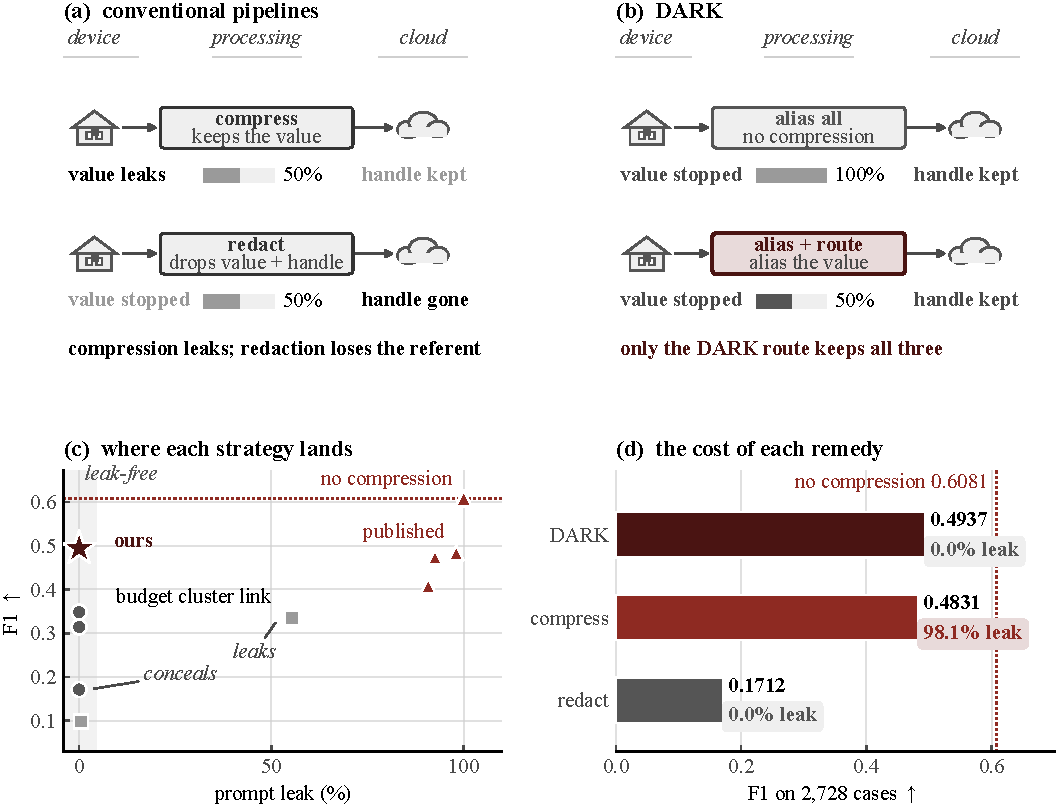
\includegraphics[width=\textwidth]{figures/fig0_teaser.pdf}
\caption{The conflict, and where each strategy lands on it. (a) A question names an account,
and the record that answers it also stores that account as a value to hide: the referent and
the protected span coincide. (b) F1 against prompt leakage for ten arms on the $2{,}728$-case
extension. Two clusters fail in opposite directions---the leak-free arms that drop protected
spans lose the referent ($0.098$ to $0.348$), and the published compressors forward the value
in $90.8\%$ to $100\%$ of cases. Only the marked point reaches $0.494$ without leaking.
(c) The two standard remedies against the routing rule; labels give the F1 gained at each
step, and the pills give the leakage that comes with it.}
\label{fig:teaser}
\end{figure*}

For this class of query, they need not compete. Figure~\ref{fig:teaser} states the conflict
and the two ways of failing it; the rest of this paper is about the third option.
The observation that makes this possible is
layout. Records in these excerpts are grouped into blocks that hold an entity's identifying
line together with the attributes recorded for it, so the queried entity and the answer to
the question about it sit in the \emph{same block} in $100\%$ of multi-entity cases and
$99.7\%$ of needle cases. A pipeline that preserves that block, and replaces the protected
values inside it with stable aliases, keeps a referential handle while never exposing the
value. Finding the block requires no answer key: the question already names the entity, and
the block is whatever contains that mention.

\paragraph{What this implies for the design.}
A single global decision cannot express it. Aliasing every protected value keeps the handle
but spends budget on sensitive records that no question component will use; deleting every
protected value removes the handle along with the value. The two axes have to be decided per
unit, and the sensitive-and-relevant cell needs an operation that neither redaction nor
deletion provides. We therefore route each unit on the pair (sensitivity, relevance) and give
each cell its own operation. Sensitive and irrelevant units are \emph{deleted}. Irrelevant
insensitive units \emph{refill} whatever budget remains. Relevant insensitive units are
\emph{kept} verbatim. Sensitive-and-relevant units are \emph{aliased} rather than deleted.
The four operations give the method its name, \textsc{DARK}: \textbf{D}elete,
\textbf{A}lias, \textbf{R}efill, \textbf{K}eep.

\paragraph{Evidence preview.}
On a 112-case benchmark spanning six public datasets, \textsc{DARK} uses $48.6\%$ of the
original tokens, leaves no protected value recoverable from the prompt, and scores F1
$0.6366$. Aliasing the whole context without compressing it scores $0.6475$ on the same
cases, a difference that is not significant; not compressing at all scores $0.7189$. The gap
that matters is against pipelines that keep the same privacy guarantee. The strongest of
those reaches $0.4308$, and in the multi-entity subset it still exposes protected values. On
a $2{,}728$-case extension, \textsc{DARK} is level with the best query-aware compressor
($0.4937$ vs.\ $0.4831$) at $0\%$ leakage against $98.1\%$. Removing the
alias-instead-of-delete rule costs $0.1795$ F1 points overall and $0.3273$ on multi-entity
cases. On the topical-question variant, where no entity can be located, it costs $+0.0013$
and is not significant. The rule acts where it is designed to act and is inert elsewhere.

\paragraph{Contributions.}
\begin{itemize}
\item \textbf{A failure mode that the compression literature does not report.} When the
queried entity is also the protected object, redundancy ordering carries almost no signal
about which record the question is about. We quantify it on $2{,}728$ cases ($47.5\%$
retention overall, $37.2\%$ on needle cases, both at a budget cut that would give an
uninformative rule $50\%$) and show that protecting the anchor \emph{line} alone repairs only
half of the gap ($57.6\%$).
\item \textbf{A training-free routing rule that does.} Sensitive-and-relevant units are
aliased rather than deleted, and relevance comes from the question by locating the record
block that contains the queried entity. The rule needs no reference answer, no training, and
no model access.
\item \textbf{An evaluation that separates privacy from utility at equal budget.} Across two
benchmark sizes, three public-benchmark variants, five budgets, two models, and two
paraphrases, \textsc{DARK} is compared with twelve published compressors and sanitizers
re-run on the same cases, with paired bootstrap intervals on every difference we report.
\end{itemize}

Section~\ref{sec:related} positions the work; Section~\ref{sec:problem} fixes notation and
the threat model; Section~\ref{sec:method} presents the routing rule;
Sections~\ref{sec:benchmark}--\ref{sec:results} describe the benchmark and the results;
Section~\ref{sec:analysis} isolates each design decision; Section~\ref{sec:discussion}
states the scope the evidence supports.
